\section{Bemeneti és kimeneti paraméterek}
\subsection{Szövegfüggő címkék}
A címke generálás egységeként egy mondatot használtunk fel. Ezt az nltk eszköz segítségével elemeztük majd az eredményekből állítottuk össze a címkéket. A címkék alapjául az aktuális fonémák szolgátak, később még ezek lettek tovább bontva idő keret szerint.A fonéma azonosítására az OneHot kódolást alkalmaztuk, azaz minden fonémát 40 értékkel azonosítottunk.

A következő szöveg függő címkéket hoztuk létre:

\begin{itemize}
	\item aktuális fonéma és az őt körülvevő két-két fonéma
	\item hangsúly
	\item megelőző és követő fonémák száma a szóban 
	\item távolság hangsúlyos fonémától mindkét irányban
	\item szó szófaja
	\item szó pozíciója a mondatban
	\item fonémák száma az aktuális szóban és két szomszédjában
	\item szavak száma a mondatba
	\item fonémák száma a mondatban
\end{itemize}

\subsection{Bemeneti paraméterek}
A szövegfüggő fonéma címkéket egészítettük ki a fonémában található időkeretek számával és a keret fonémán belüli elhelyezkedésével. Így a kerethez tartozó 215 bemeneti paraméter az alábbiakból tevődik össze:


\begin{minipage}{0.5\textwidth}
	\begin{itemize}
		\item 0-200 A 40-40 paraméter a kvinfón(2-1-2) fonémáira
		\item 200-213 további szövegfüggő címkék
		\item 213 A fonémán belüli időkeretek száma
		\item 214 A keret elhelyezkedése a fonémán belül
	\end{itemize} 
\end{minipage} \hfill
\begin{minipage}{0.5\textwidth}
	\centering
	Címkék létrehozásának folyamata
	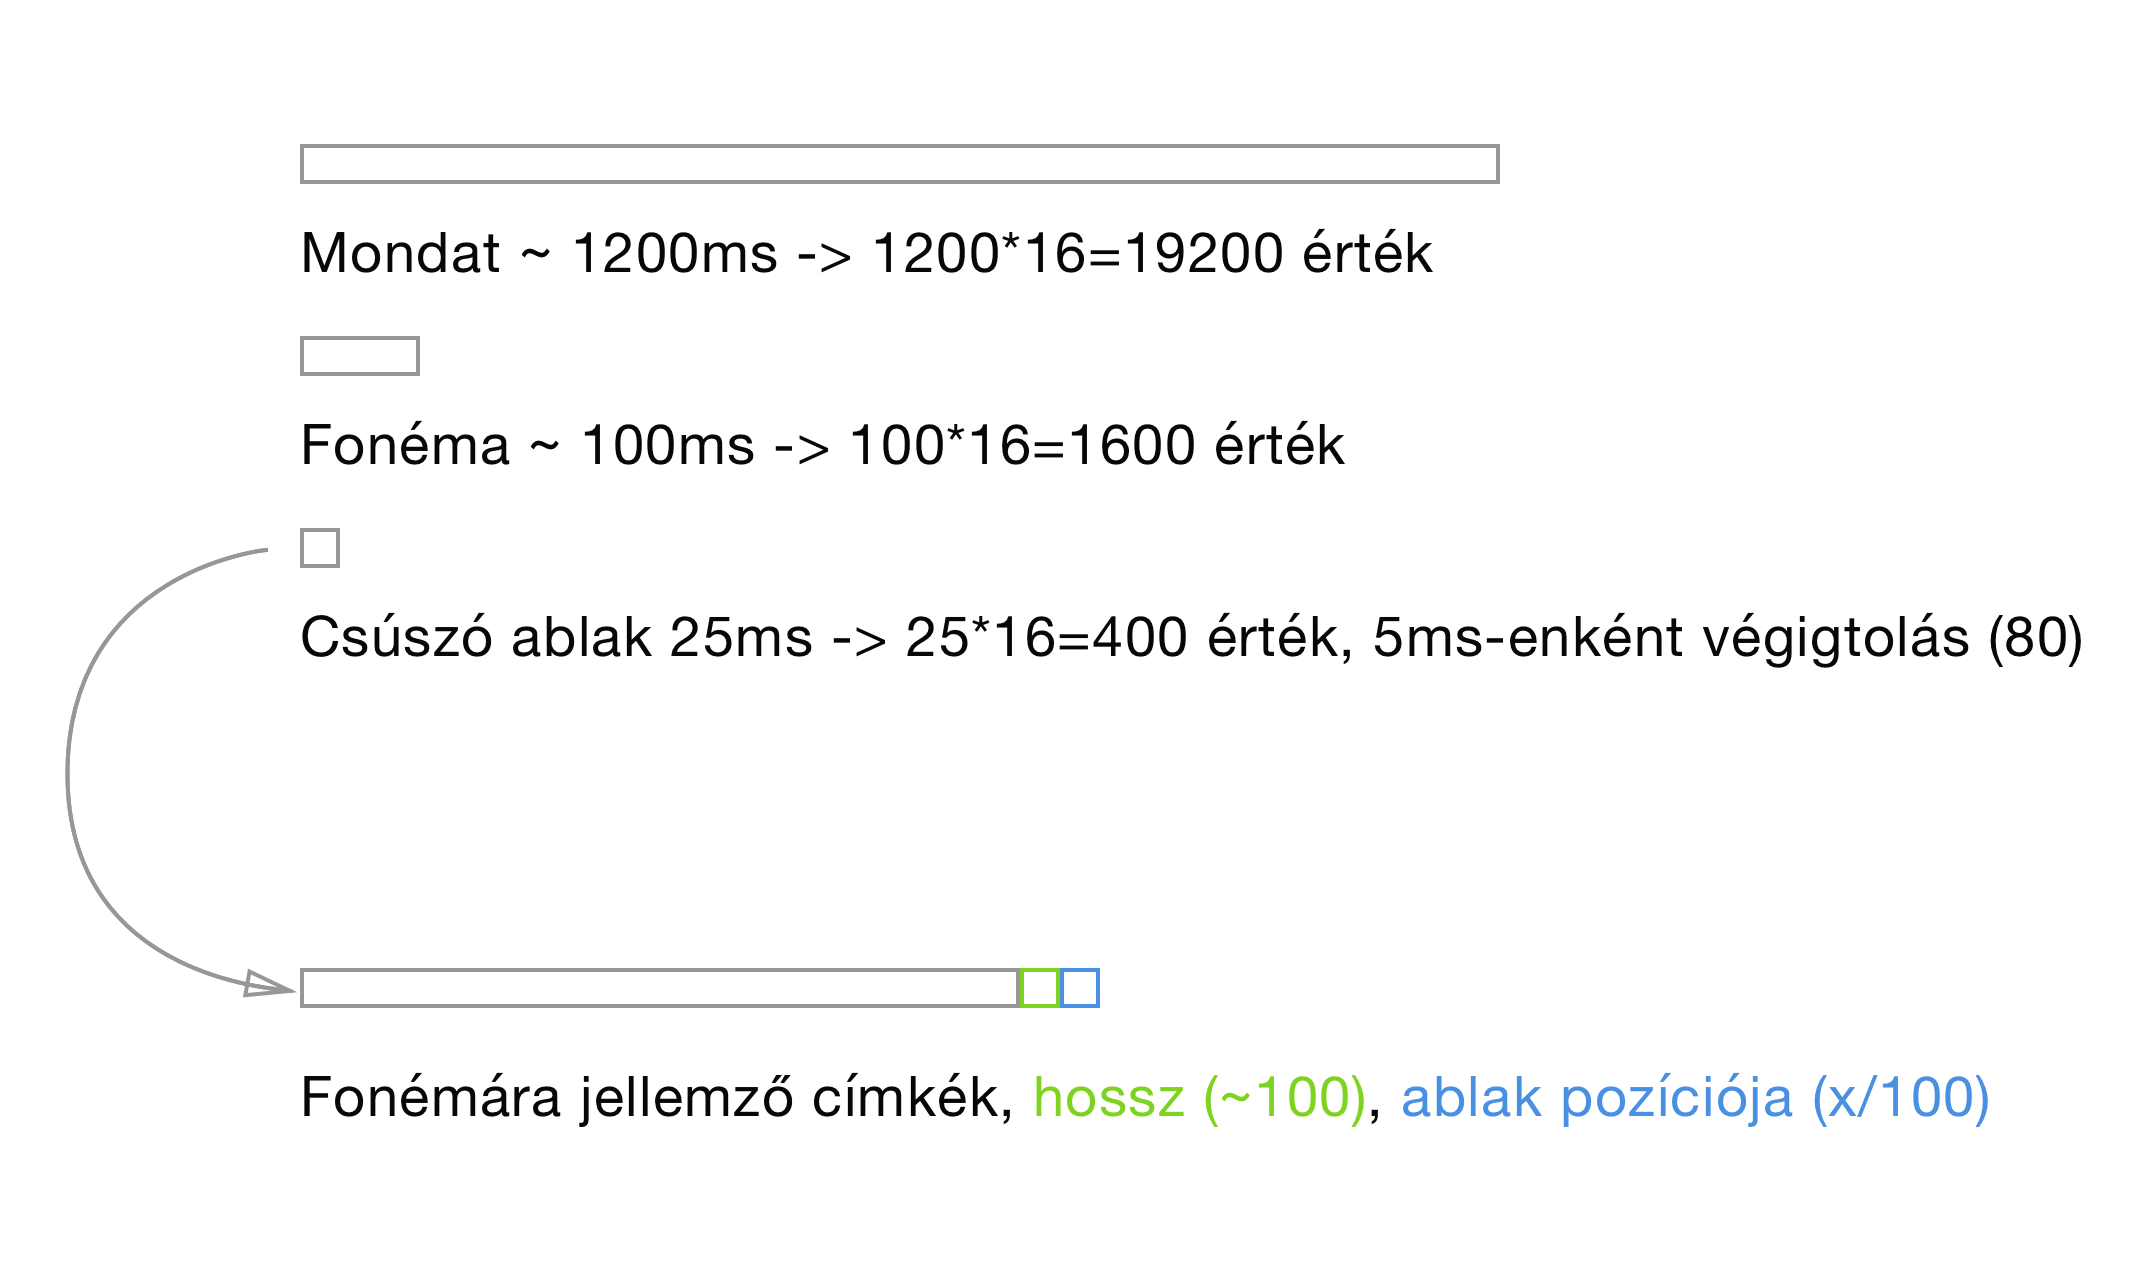
\includegraphics[width=5cm,keepaspectratio]{tag_struct}
\end{minipage} \hfill
\subsection{Kimeneti paraméterek}
Az előző felsorolást folytatva az aktuális időkerethez tartozó elvárt a kimenet paraméterek a következők:

 
\begin{itemize}
	\item 215 a keret hangmagasság értéke
	\item 216-242 a Mel-Cepstrum 26 paramétere
	\item 242 a fonémán belüli keretek száma
\end{itemize}
\subsection{Spektrális és gerjesztési paraméterek}
Mint említettük a prediktálás alapja a spektrális és gerjesztési paraméterek megadása keretenként. Ezen paraméterek segítségével a PyPSTK \ [2] python csomag használásával állíthatjuk elő az audio kimenetet, valamint hasonlóképpen ezt a csomagot használjuk az adataink a tiszta hangból való előállítására.
\subsubsection{Mel-Cepstrum}
A paraméterek előállításához, visszafejtéséhez a PyPSTK Mel-Cepstrum alapú algoritmusát alkalmazzuk. Az algoritmust T. Fukada és társai fejlesztették ki.\ [3]


Ezzel a metódussal természetesen adatvesztést kapunk, azonban az így előállított hang még megfelel a mércéinknek. Viszont az általunk generált kimenetek értékelésénél ezt figyelembe kell vennünk.

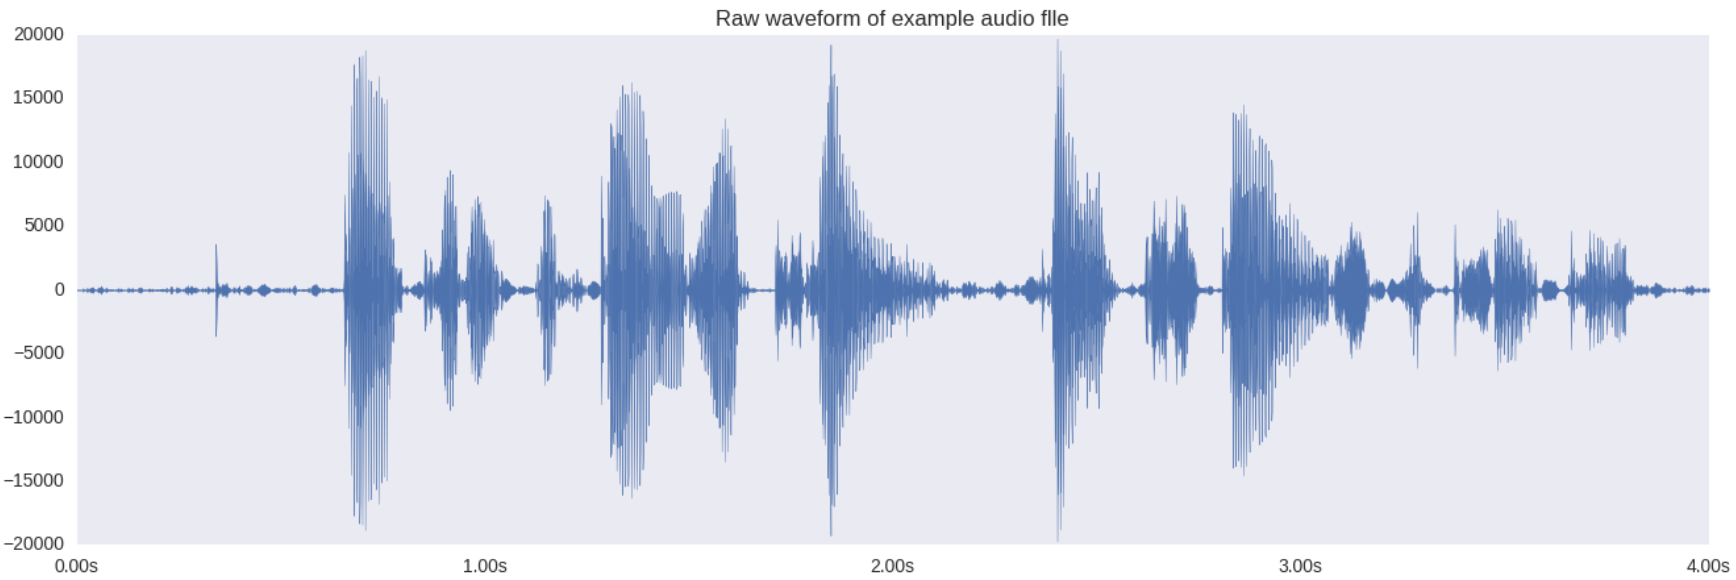
\includegraphics[width=\textwidth,keepaspectratio]{audio_raw}

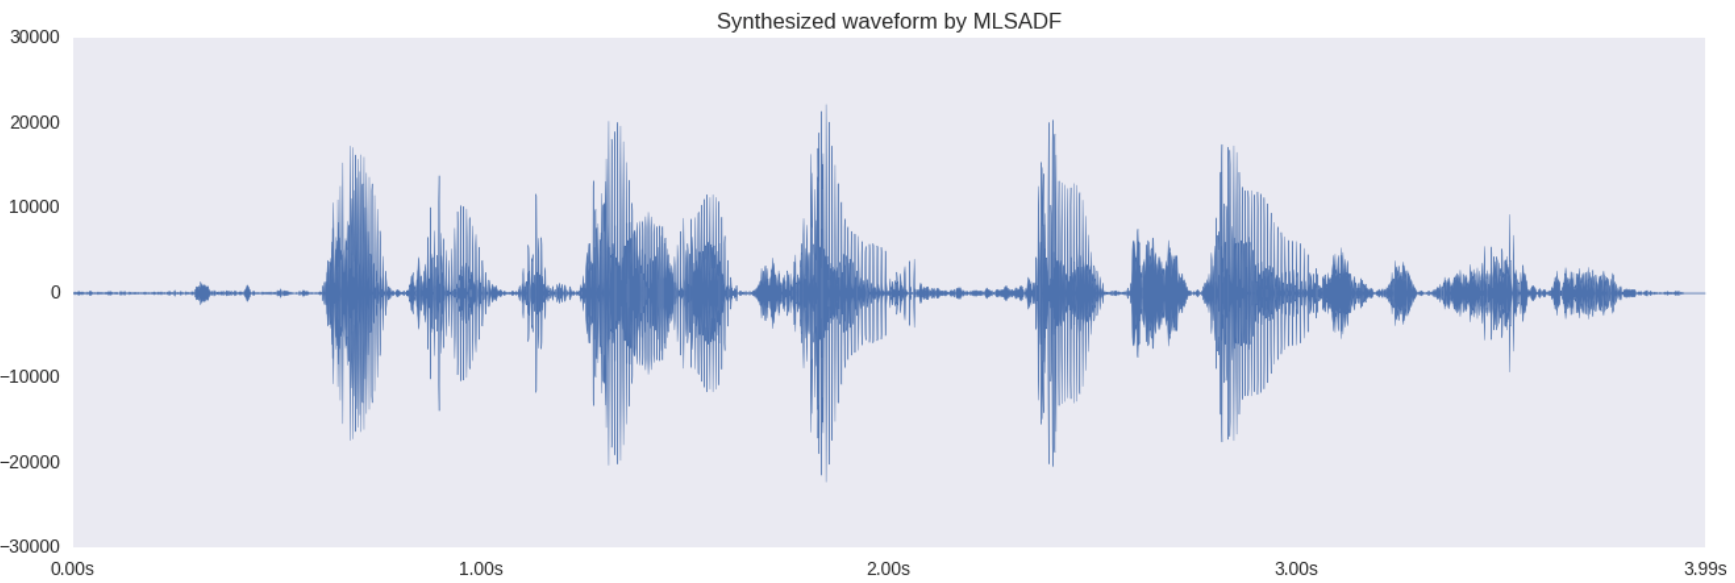
\includegraphics[width=\textwidth,keepaspectratio]{audio_mc}